\documentclass[11pt]{scrartcl}

\usepackage[hyphens]{url}
\usepackage{float}
\usepackage{graphicx}

\title{
  \textbf{\large Database Tuning -- Assignment 1}\\
  Uploading Data to the Database
}

\author{
 A3\\
 \large Platzer Hugo, 1421579 \\
 \large Strohmeier Mario, 1422959 \\
}

\begin{document}

\maketitle

\subsection*{Straightforward Implementation}

  \paragraph{Implementation}

  Every tuple gets inserted individually, by iterating over each line from the tsv file and executing the insert.

{\small
\begin{verbatim}
    "INSERT INTO auth (name, pubid) values (?, ?)"
\end{verbatim}
}

  \subsection*{Efficient Approach 1: (Batch/Bulk Insert)}

  \paragraph{Implementation}

  With this method, we don't execute the insert for each tuple seperatly. We keep adding tuples to a batch, until it is big enough or there are no tuples left. After the batch is big enough, we execute the insert for our whole batch.\\\\
  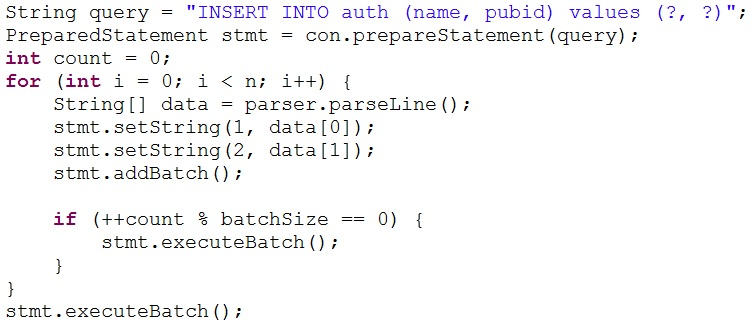
\includegraphics{batch.jpg}

  \paragraph{Why is this approach efficient?}

  This approach is more efficent, since we don't need to write a log for every single insert. This frees a lot of disk access time. Furthermore there is a lot less connection overhead, because the packets we send are bigger.\footnote{\url{https://dbresearch.uni-salzburg.at/teaching/2016ws/dbt/dbt_01-handout-1x1.pdf}, Page 23-27}

  \paragraph{Tuning principle}

  start-up costs are high; running costs are low

    \subsection*{Efficient Approach 2: (SQL COPY statement)}

  \paragraph{Implementation}

  Our data is in the form of a TSV file meaning each line contains a
  (auth, pubid) tuple, the two values separated by a TAB character. Data like this can be
  directly loaded into the Postgres database by using the COPY command. This can be
  done using the psql prompt:
  
  {\small
\begin{verbatim}
  \copy auth from ~/dbtuning/data/auth.tsv DELIMITER e'\t'
\end{verbatim}
}

It can also be done with JDBC using the CopyManager class and a FileReader
for the input:

{\small
\begin{verbatim}
  public static void insertCopyFrom(Connection con, String filename, int n)
          throws SQLException, IOException {
      CopyManager copyManager = new CopyManager((BaseConnection) con);
      FileReader fileReader = new FileReader(filename);
    
      copyManager.copyIn("COPY auth from STDIN WITH DELIMITER '\t'", fileReader);
  }
\end{verbatim}
}

  \paragraph{Why is this approach efficient?}

  Compared to the straightforward approach, this creates one ''query''
  for the whole file, avoiding excessive network roundtrips and minimizing
  data overhead (query parameters). The database systems' insert code
  is only called once. Also it prevents lots of unneccessary
  logfile access. Most of the file/data processing
  is done on the server, this might also be more efficient than
  processing the file manually line per line in Java.
  
  
  \subparagraph{References:}
  
  \begin{itemize}
  
  \item{Postgres Documentation, COPY statement}
  
  \url{https://www.postgresql.org/docs/9.2/static/sql-copy.html}
  
  \item{Stackoverflow, 'How to copy data from file to Postgres using JDBC'}
  
  \url{https://stackoverflow.com/questions/6958965/
  how-to-copy-a-data-from-file-to-postgresql-using-jdbc}
  
  \end{itemize}

  \paragraph{Tuning principle}
  
  ''Start-Up Costs Are High; Running Costs Are Low''

  \subsection*{Runtime Experiment}

  \begin{table}[H]
  \begin{tabular}{l|r}
    Approach & Runtime [sec] \\
    \hline
    Straightforward & 11400 \\
    Batch / Bulk Insert & 120 \\
    SQL COPY statement & 8   
  \end{tabular}
  \end{table}

  \bigskip

  \noindent Notes:
  \begin{itemize}
  \item The provided ''biber'' database server was used as target for
  uploading the data, tsv files were stored on the cosy user account home folder,
  the program was run from a machine at the computer room of the facility.
  
  \item For the straightforward approach, only 10000 records were uploaded,
  we scaled the 38 sec. taken linearly to approximate the time taken for all $\approx 3$ mio records.
  
  \item For the batch insert, we chose a batch size of 1000 since experiments showed
  larger batch sizes do not give further speedup.
\end{itemize}

  \subsection*{Time Spent on this Assignment}

  Time in hours per person: {\bf 3.14159}

\end{document}
